\section{Machine Perception Services}
\label{sec:mps}

We provide a range of foundational machine perception capabilities upon which research partners can build their projects. We expect these capabilities to be provided in a similar form on any future AR device.

These capabilities are exposed as Machine Perception Services (MPS) enabled by a set of proprietary algorithms that are designed for \AriaDevices{} and provide superior accuracy and robustness on the recorded data compared to current off-the-shelf open source solutions.


MPS is provided by post-processing VRS recordings on Meta's backend servers. To use the service, \ProjectAria research partners upload the recording, and, later on, can download the results. Furthermore, we include MPS output in public Aria-based datasets making it available to the broader community. 

Please refer to the \ProjectAria{} documentation site \cite{ariadocs} for more information about Aria MPS, the output format and their specifications, and an overview over the tooling available to visualize and make use of the data.


\begin{figure}[t]
    \centering
{\setlength{\fboxsep}{0pt}%
\setlength{\fboxrule}{0.5pt}%
\fbox{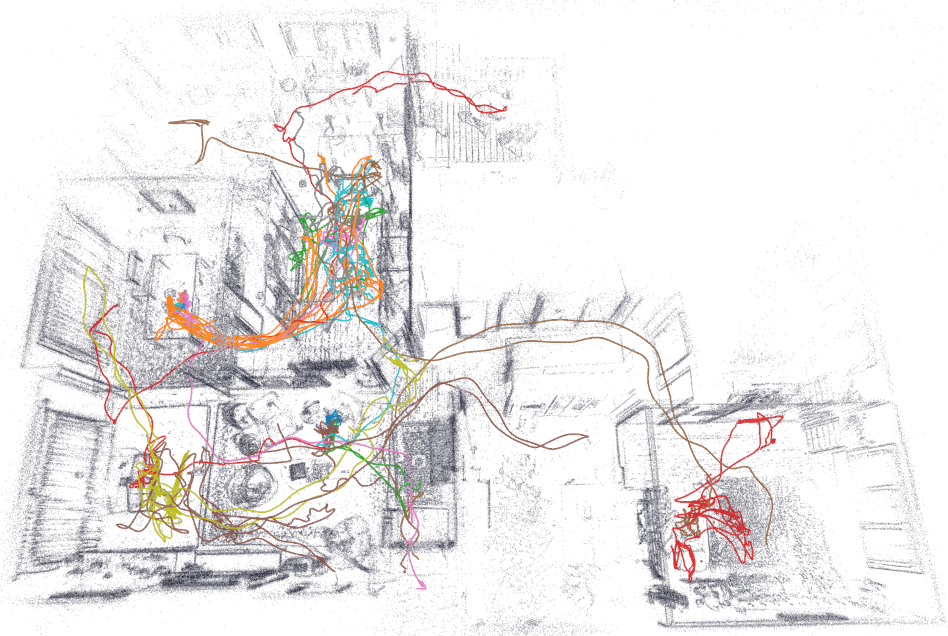
\includegraphics[width=0.99\linewidth]{images/mps_static_2.png}}}
    \caption{Closed-loop trajectories and semi-dense point clouds of 18 recordings of Aria Pilot Dataset \cite{ariapilot} collected in the same home space.}
    \label{fig:mps_static}
\end{figure}


\subsection{Trajectories}
\label{sec:trajectories}

A highly accurate 6-DoF device trajectory is the foundation to understand the geometric relation of the device and its wearer to the environment. Device trajectories are generated by a state-of-the-art VIO and SLAM system -- similar to what can be expected on future AR and VR HMD's -- followed by offline post-processing and refinement. We use multiple of the available sensors (including cameras, IMUs, GNSS, Wi-Fi, and barometer) to improve accuracy and robustness, and further take advantage of precise knowledge of the sensor models, timing, and rigidity of \AriaDevices{}. This allows us to robustly localize the device even under the often challenging conditions that occur with real-world data - such as fast motion, low or highly dynamic lighting, partial or temporary occlusion of the cameras, as well as a wide range of static and dynamic environments. 

We provide two types of trajectories as output, open loop and closed loop.  The \textit{open loop trajectory} is a high frequency (1\,kHz) odometry estimation, computed strictly causally with a real-time-compatible method. The accumulated translation drift of this open loop trajectory is no more than 0.4\% of the distance traveled, and usually significantly less. The \textit{closed loop trajectory} is a 1\,kHz trajectory estimated in post-processing. It is fully optimized and provides poses in a single frame of reference. We also provide the ability to jointly process multiple recordings, placing them into a common coordinate frame, as shown in Figure~\ref{fig:mps_static}. Closed loop trajectories have a typical global RMSE translation error of no more than 1.5\,cm in room-scale scenarios. 


\subsection{Online Calibration}
\label{sec:onlinecalib}

Accurate device calibration is essential to enable high geometric accuracy for downstream 3D perception tasks.
Even though \AriaDevices{} are built to be as rigid as possible, device calibration parameters are not perfectly constant over time due to temperature changes, aging, and external forces applied to the device. 
Figure~\ref{fig:mps_online_calib} shows an example where taking off the device after wearing causes around 25\,arc\-min instantaneous rotational deformation between the left and right Mono Scene cameras (corresponding to roughly 1.5~pixel shift in the images). 
To account for this, we estimate the time-varying intrinsic and extrinsic calibrations of cameras and IMUs as part of MPS, and make the result available to researchers. 


\begin{figure}[tbp]
    \centering
    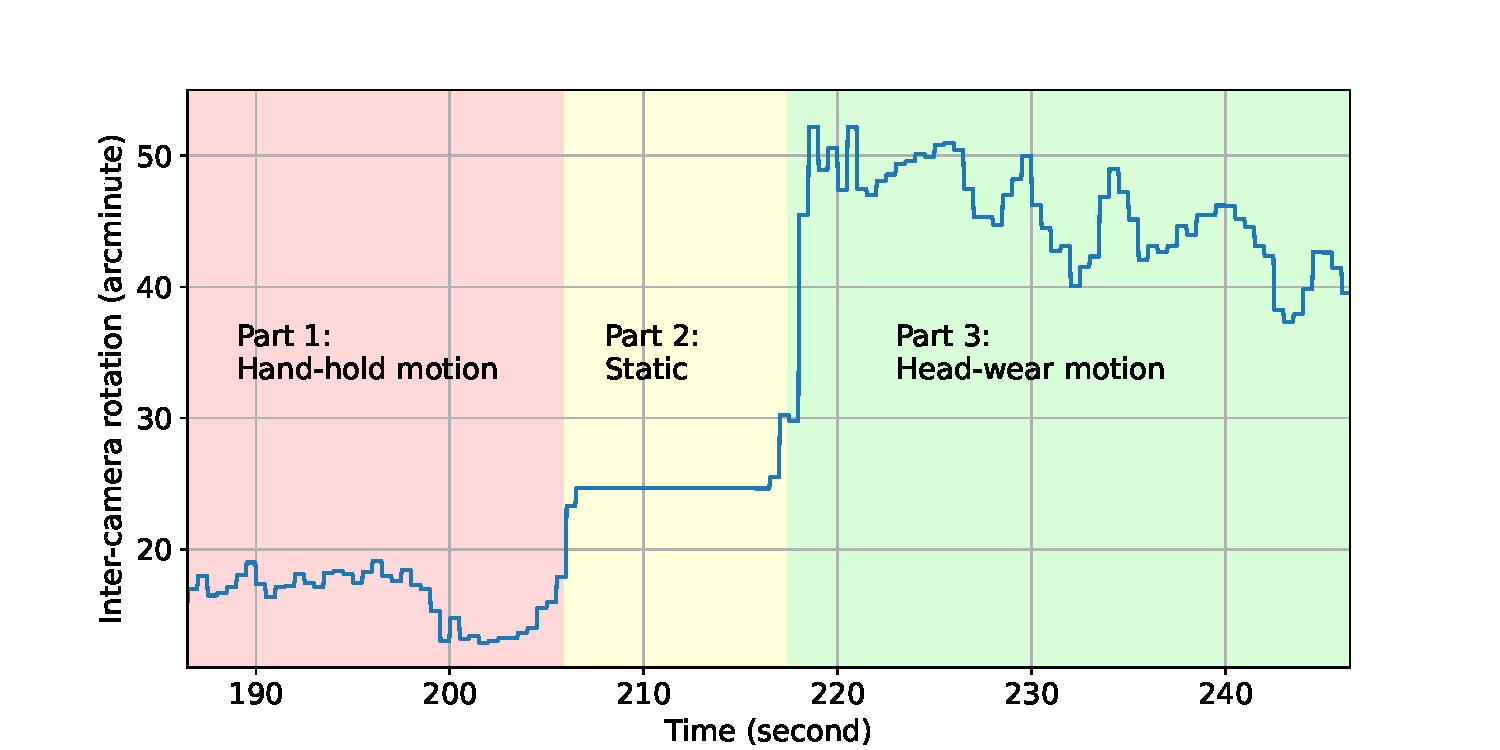
\includegraphics[width=\linewidth]{images/mps_online_calib.pdf}
    \caption{Example of rotational deformation between left and right Mono Scene cameras, estimated by MPS. The recording used for this figure contains 3 sections: hand-held motion, no motion, and head-worn motion. The effect of external force applied to the glasses when worn on the head is clearly visible.}
    \label{fig:mps_online_calib}
\end{figure}

\subsection{Semi-Dense Point Cloud}
\label{sec:semi-dense}
To provide an intuitive understanding of the environment a recording was taken in, we compute semi-dense tracks and point clouds as part of MPS; see Figure~\ref{fig:mps_static} for an example.  Similar to the odometry trajectory, these tracks are computed causally and provide an accurate -- though partial -- reconstruction of the static portion of the environment. We also provide the sets of all 2D observations that were used to triangulate each 3D point. Tracks are obtained by continuously spawning new points in images-regions with high gradient, and tracking these over time and across the left/right Mono Scene camera using affine-invariant photoconsistency of local patches. Finally, the 3D point clouds are post-processed and placed into the global frame of reference that is defined by the closed loop trajectories.

\subsection{Eye Gaze Tracking}

Gaze direction is an important indicator of a wearer's attention, and will likely be one of the crucial inputs to context-aware, personalized AI agents.
We compute and provide eye gaze from the \AriaDevice{} eye tracking cameras, estimating a single per-frame 3D ray anchored to the central pupil frame, also called a cyclopean eye frame \footnote{The central pupil frame origin is defined at the midpoint between the left and right pupils.}. We also provide confidence intervals, as eye tracking accuracy can vary by situation and user. 

Furthermore, the Aria companion app described in Section \ref{sec:recordingtools} implements the option to capture personalized eye calibration - this allows to improve the accuracy of eye gaze tracking by compensating for user-specific biases. With the current model, we observe a median gaze ray error of 1.5\textdegree\ after applying the personalized calibration.

\begin{figure}[tbp]
    \centering
    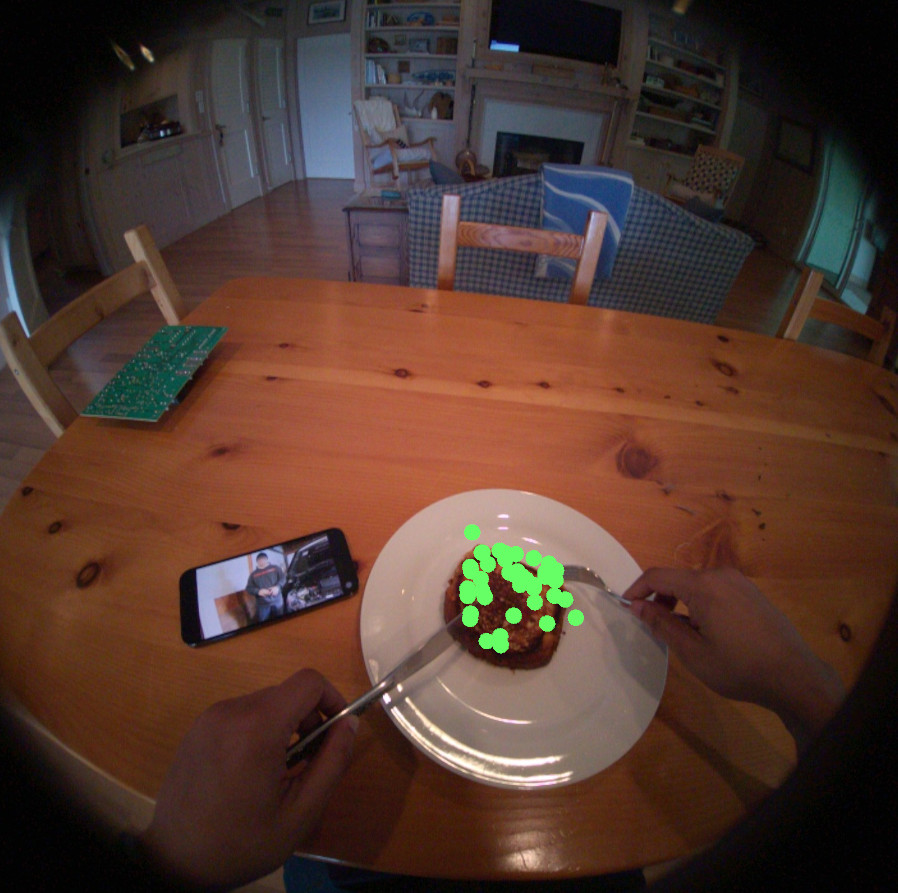
\includegraphics[height=0.442\linewidth]{images/mps_gazeimg_example.jpg}%
\hfill%    
{\setlength{\fboxsep}{0pt}%
\setlength{\fboxrule}{0.5pt}%
\fbox{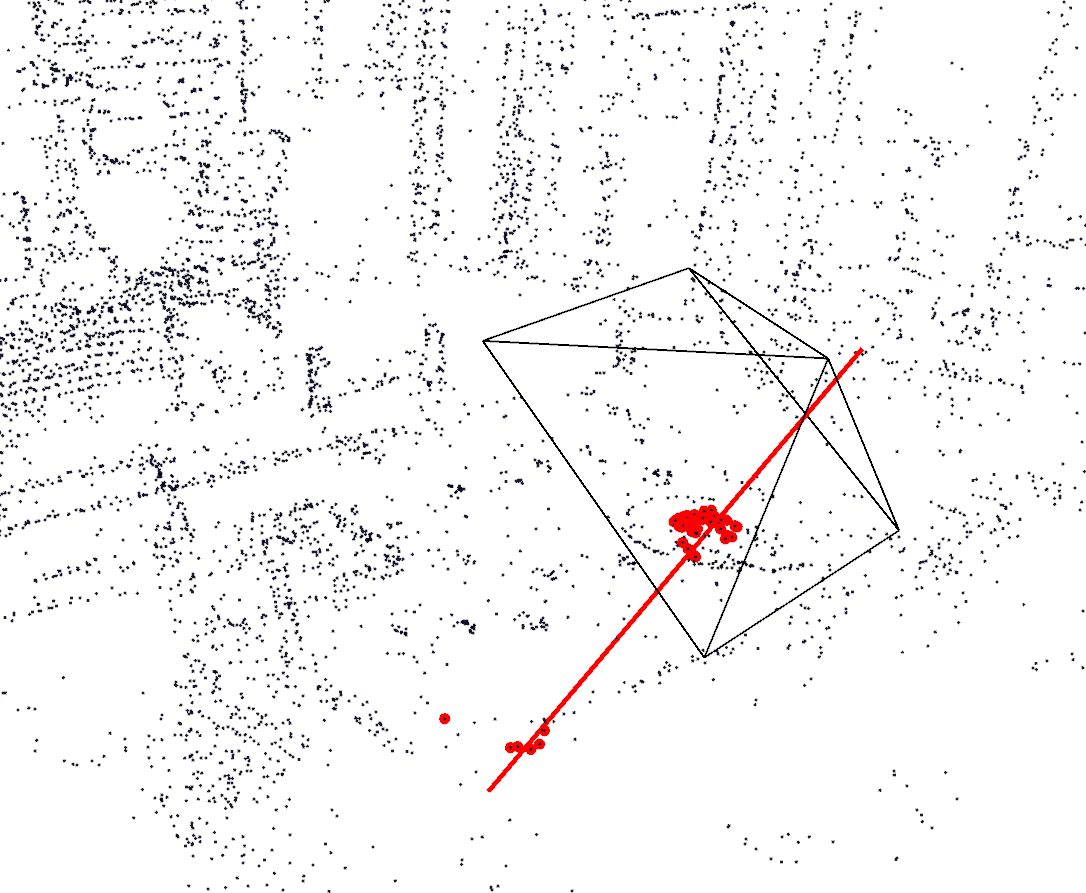
\includegraphics[height=0.442\linewidth]{images/mps_gaze_example.png}}}
    \caption{Eye gaze computed on a recording in which the user is looking at the food on their plate. Left: The RGB image with semi-dense points that are close to the gaze ray projected as green dots. Right: The \AriaDevice{} pose (shown as RGB camera frustum), semi-dense points, and eye gaze ray. Semi-dense points close to the gaze ray are highlighted in red.}
    \label{fig:mps_gaze}
\end{figure}

